\addchap{Anhang A}
\textbf{\LARGE Baustein ''Main''}
\setcounter{chapter}{1}
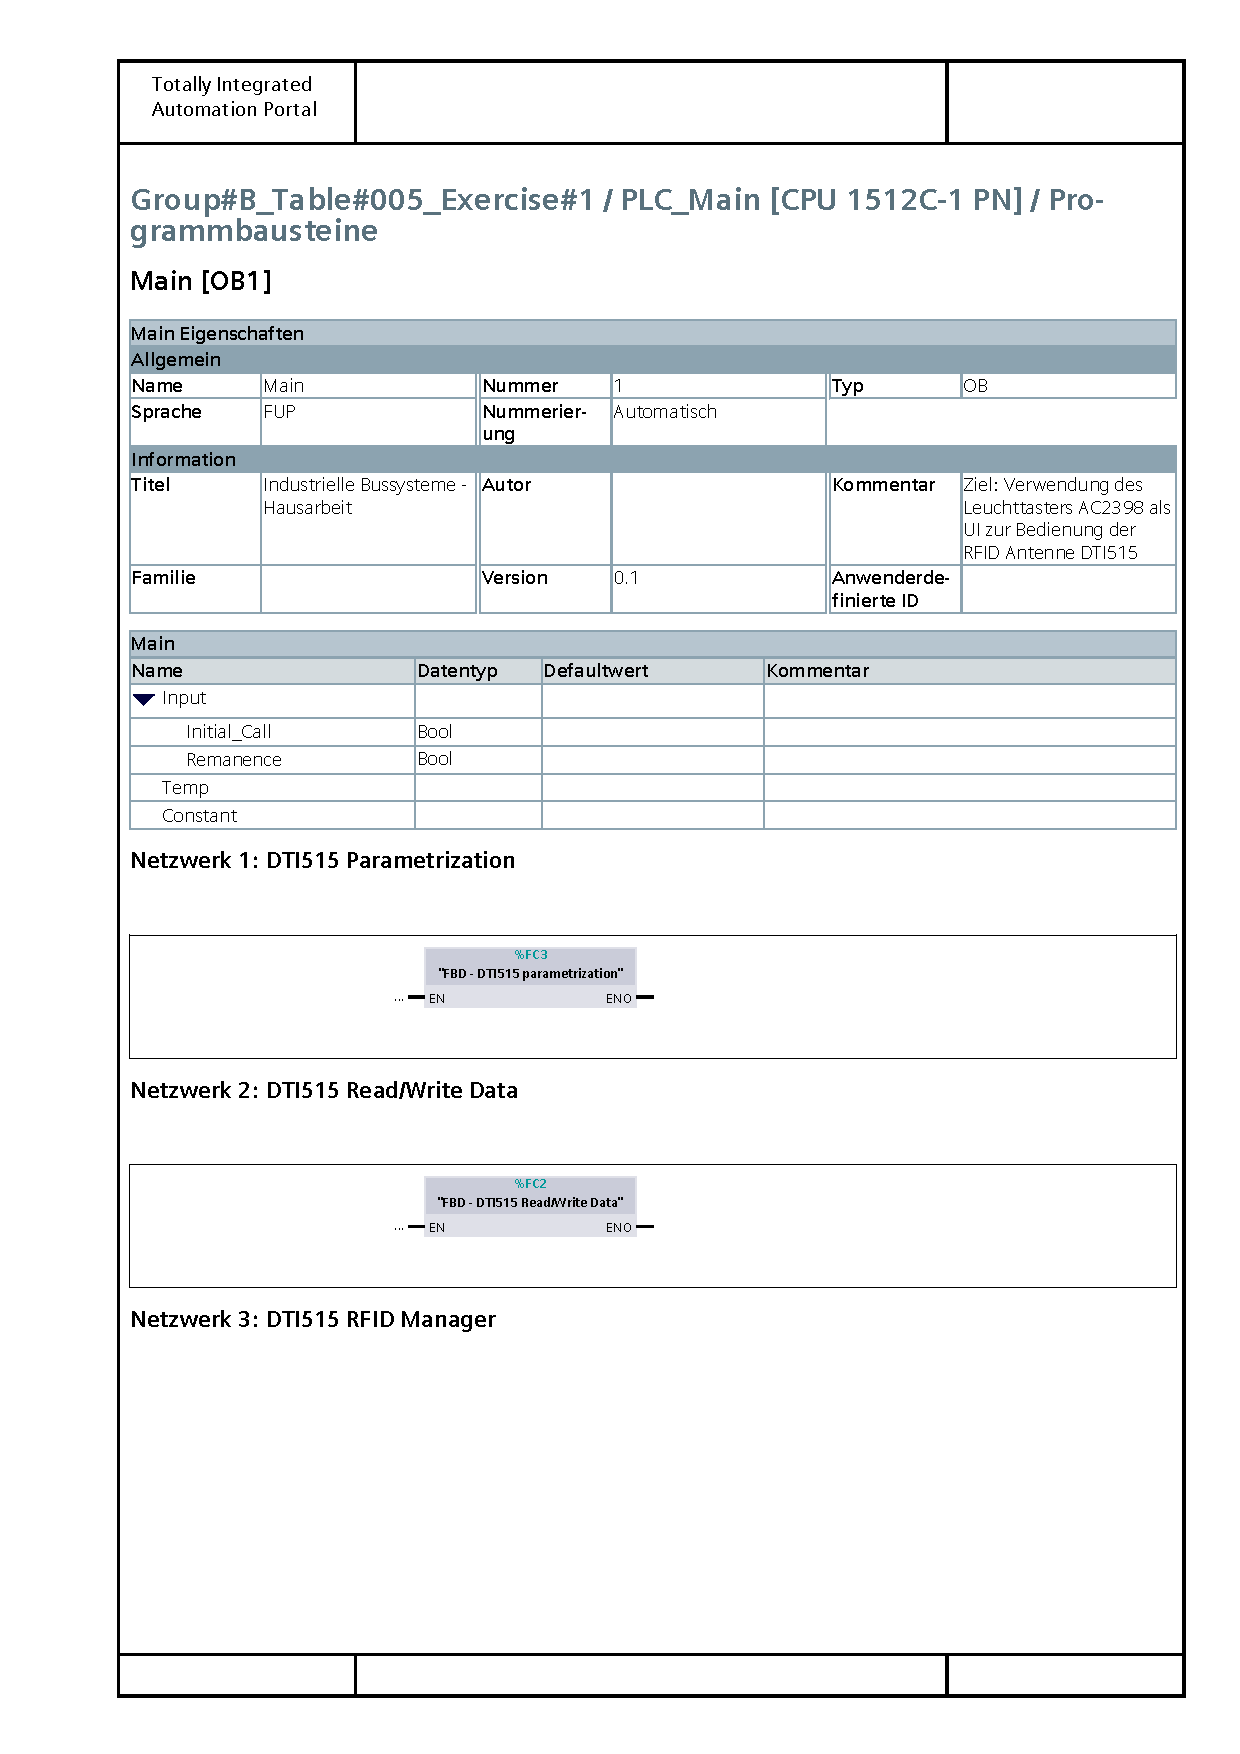
\includepdf[pages=-, scale=0.9]{doc/Main.pdf}
\addchap{Anhang B}
\textbf{\LARGE Funktion ''FBD\_DTI515 parametrization''}
\setcounter{chapter}{2}
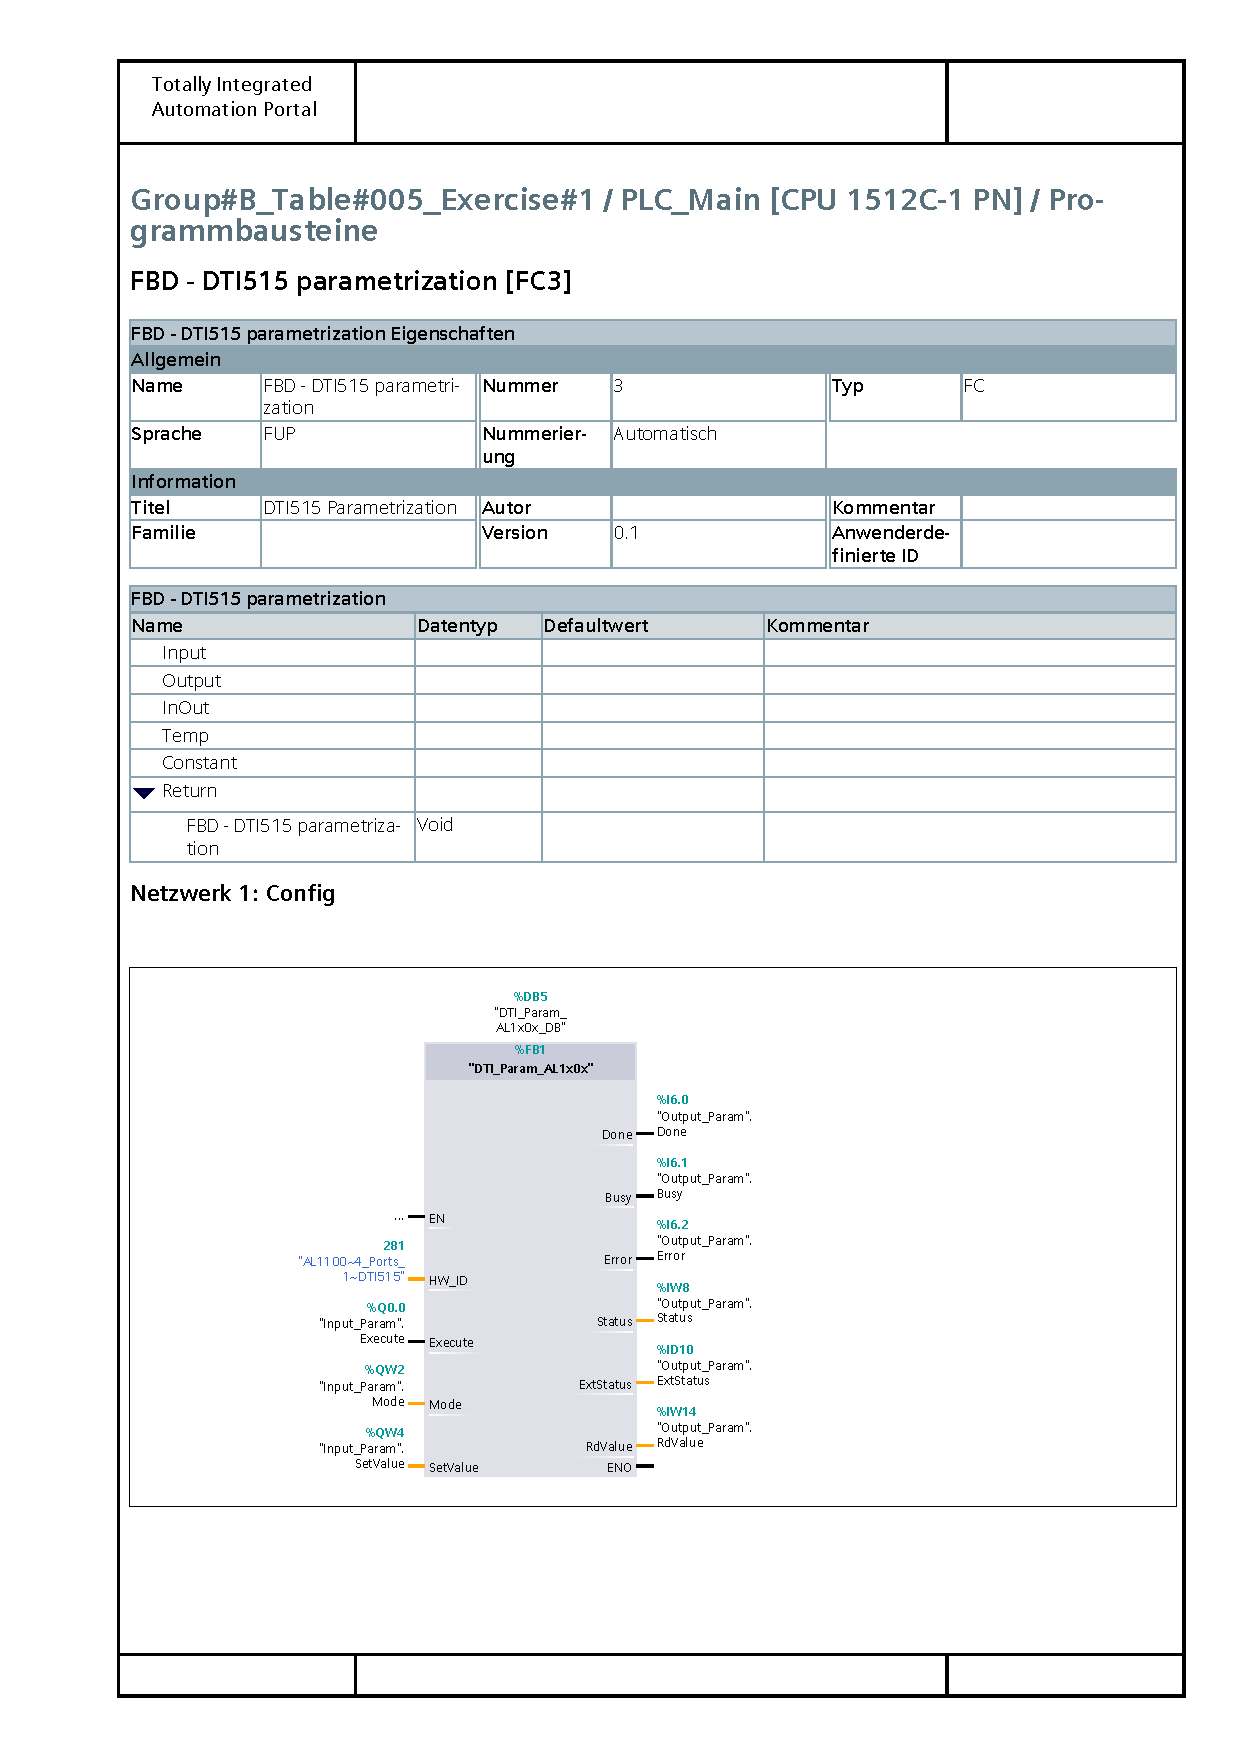
\includepdf[pages=-, scale=0.9]{doc/FBD_DTI515 parametrization.pdf}
\addchap{Anhang C}
\textbf{\LARGE Funktion ''FBD\_DTI515 Read-Write\_Data''}
\setcounter{chapter}{3}
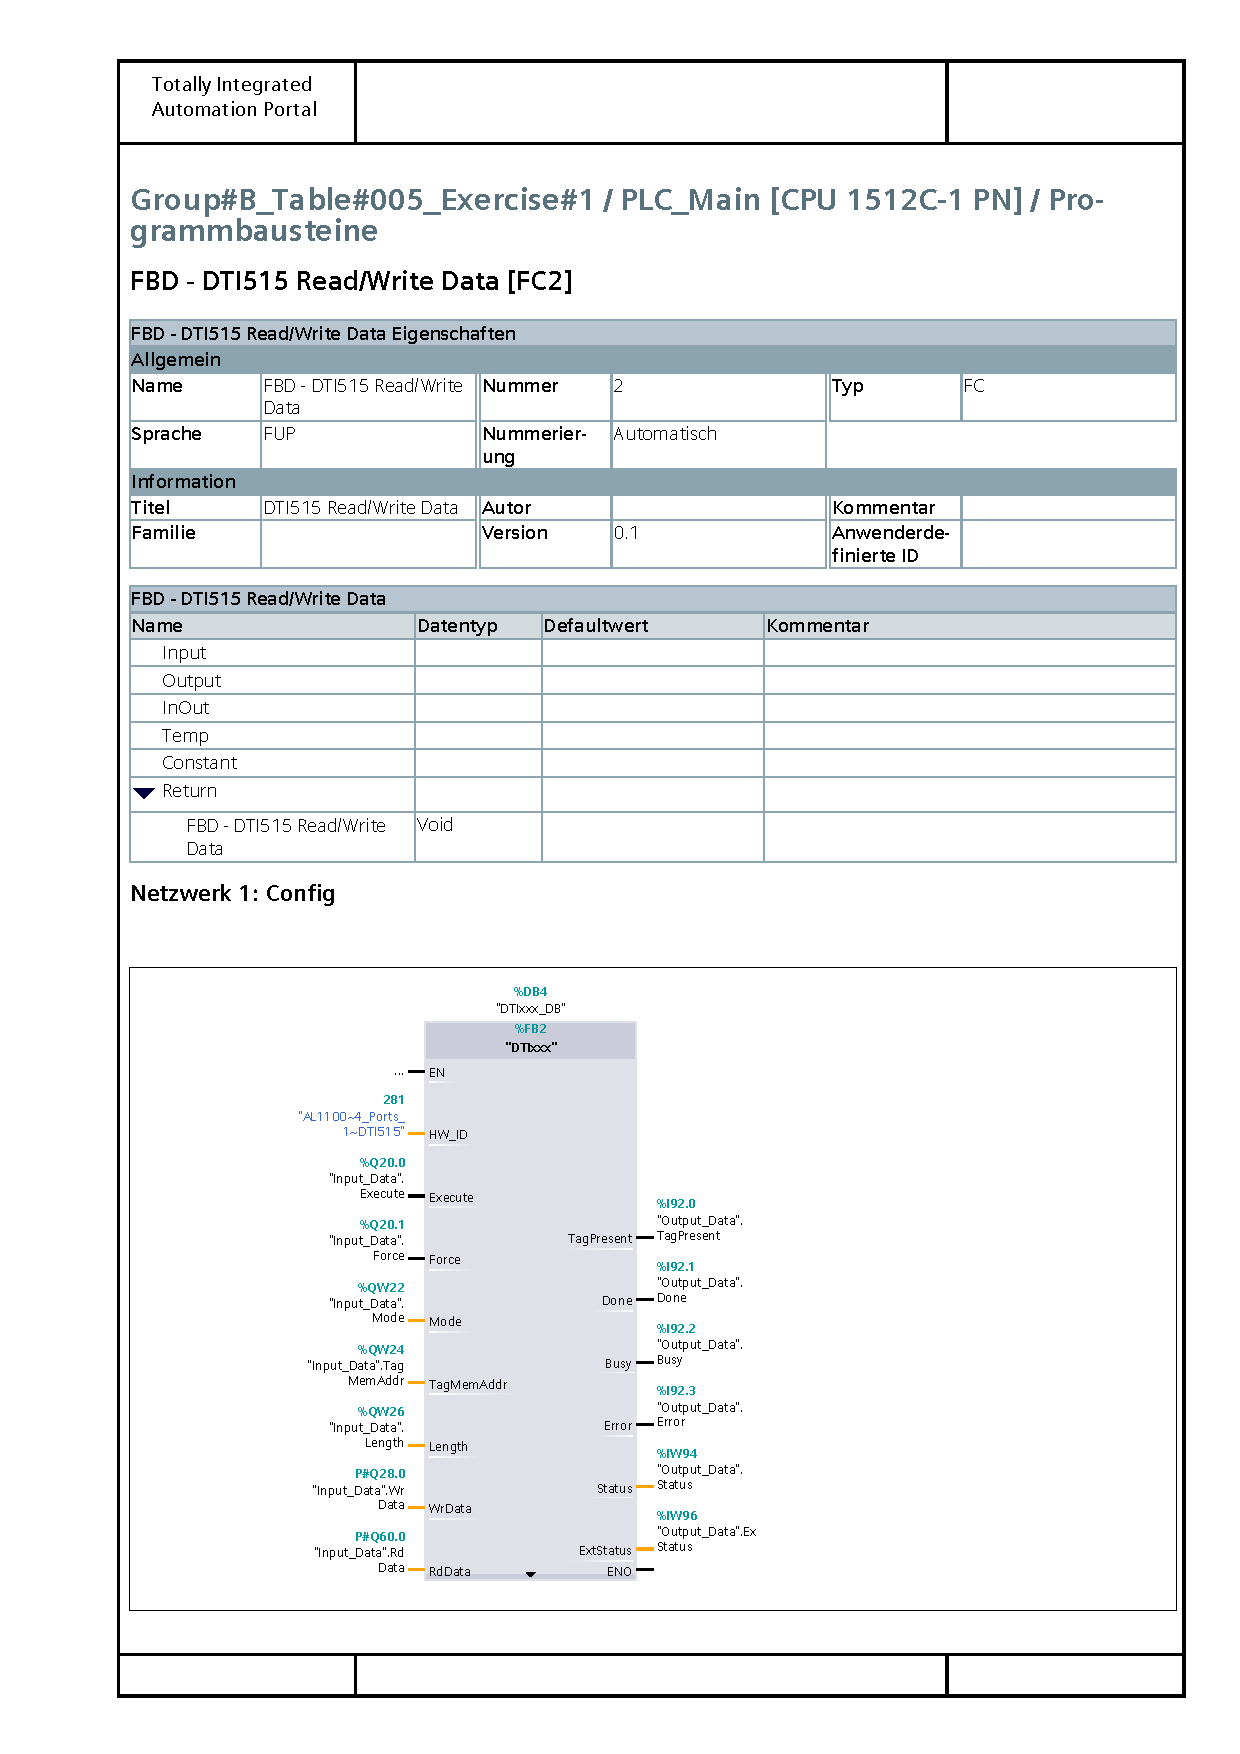
\includepdf[pages=-, scale=0.9]{doc/FBD_DTI515 Read-Write_Data.pdf}
\addchap{Anhang D}
\textbf{\LARGE Funktionsbaustein ''FB\_RFID\_Manager''}
\setcounter{chapter}{4}
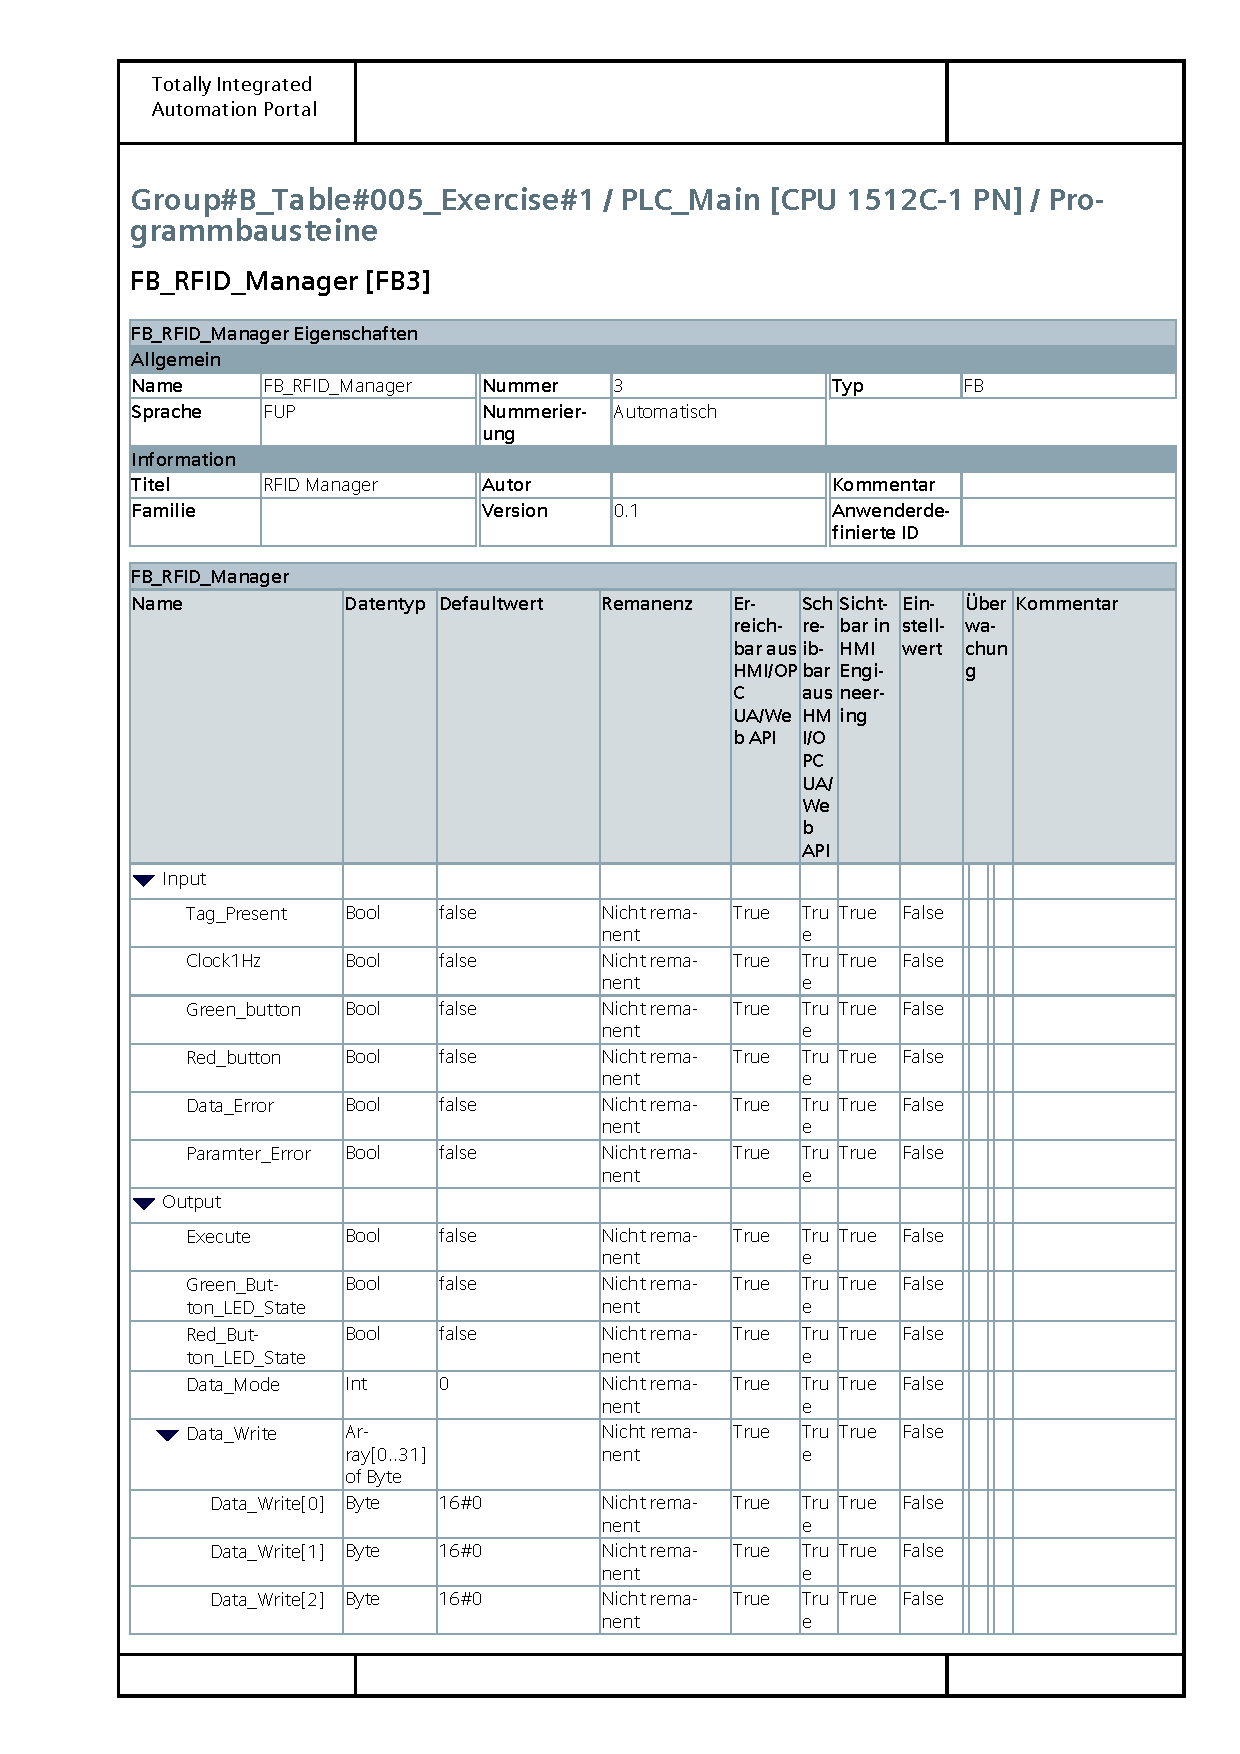
\includepdf[pages=-, scale=0.9]{doc/FB_RFID_Manager.pdf}
%------------------------------------------------------------------
%-----------------------------------------------------------------------------------
% Layout of Template
%\section{Details}
%\addchap{Anhang B}
%\addchap{Anhang C}
%\addchap{Anhang D}
%\setcounter{chapter}{4}
%\setcounter{section}{0}
%\setcounter{table}{0}
%\setcounter{figure}{0}
%\section{Einbinden von PDF-Seiten aus anderen Dokumenten}
%Auf den folgenden Seiten wird eine Möglichkeit gezeigt, wie aus einem anderen PDF-Dokument komplette Seiten übernommen werden können. Der Nachteil dieser Methode besteht darin, dass sämtliche Formateinstellungen (Kopfzeilen, Seitenzahlen, Ränder, etc.) auf diesen Seiten nicht angezeigt werden. Die Methode wird deshalb eher selten gewählt. Immerhin sorgt das Package \textit{\glqq pdfpages\grqq}~für eine korrekte Seitenzahleinstellung auf den im Anschluss folgenden \glqq nativen\grqq~\LaTeX-Seiten.
%Eine bessere Alternative ist, einzelne Seiten mit \textit{\glqq$\backslash$includegraphics\grqq}~einzubinden. Z.B. wenn Inhalte von Datenblättern wiedergegeben werden sollen.
%\includepdf[pages={2-4}]{docs/EingebundenesPDF.pdf}